\documentclass[12pt, a4paper]{article}

\usepackage[czech]{babel}
\usepackage{lmodern}
\usepackage[utf8]{inputenc}
\usepackage[T1]{fontenc}
\usepackage[pdftex]{graphicx}
\usepackage{amsmath}
\usepackage[hidelinks,unicode]{hyperref}
\usepackage{float}
\usepackage{listings}
\usepackage{tikz}
\usepackage{xcolor}
\usepackage{tabularx}
\usepackage[final]{pdfpages}
\usepackage{syntax}


\definecolor{mauve}{rgb}{0.58,0,0.82}
\usetikzlibrary{shapes,positioning,matrix,arrows}

\newcommand{\img}[1]{(viz obr. \ref{#1})}

\definecolor{pblue}{rgb}{0.13,0.13,1}
\definecolor{pgreen}{rgb}{0,0.5,0}
\definecolor{pred}{rgb}{0.9,0,0}
\definecolor{pgrey}{rgb}{0.46,0.45,0.48}


\lstdefinestyle{flex}{
    frame=tb,
    aboveskip=3mm,
    belowskip=3mm,
    showstringspaces=false,
    columns=flexible,
    basicstyle={\small\ttfamily},
    numbers=none,
    numberstyle=\tiny\color{black},
    keywordstyle=\color{black},
    commentstyle=\color{black},
    stringstyle=\color{black},
    breaklines=true,
    breakatwhitespace=true,
    tabsize=3
}

\lstset{
    frame=tb,
    language=C,
    aboveskip=3mm,
    belowskip=3mm,
    showstringspaces=false,
    columns=flexible,
    basicstyle={\small\ttfamily},
    numbers=none,
    numberstyle=\tiny\color{gray},
    keywordstyle=\color{blue},
    commentstyle=\color{pgreen},
    stringstyle=\color{mauve},
    breaklines=true,
    breakatwhitespace=true,
    tabsize=3
}


\let\oldsection\section
\renewcommand\section{\clearpage\oldsection}

\begin{document}
	% this has to be placed here, after document has been created
	% \counterwithout{lstlisting}{chapter}
	\renewcommand{\lstlistingname}{Ukázka kódu}
	\renewcommand{\lstlistlistingname}{Seznam ukázek kódu}
    \begin{titlepage}

        \centering

        \vspace*{\baselineskip}
        \begin{figure}[H]
        \centering
        
\includegraphics[width=7cm]{img/fav-logo.jpg}
        \end{figure}

        \vspace*{1\baselineskip}

        \vspace{0.75\baselineskip}

        \vspace{0.5\baselineskip}
        {Semestrální práce z předmětu KIV/FJP}

        {\LARGE\sc Tvorba vlastního překladače\\}
        {\sc pro vlastní jazyk C-{}-\\}

        \vspace{4\baselineskip}

        \vspace{0.5\baselineskip}

        {\sc\Large Jindřiška Reismüllerová \\}
        \vspace{0.5\baselineskip}
        {A20N0104P}

        {\sc\Large Stanislav Král \\}
        \vspace{0.5\baselineskip}
        {A20N0091P}

        \vfill

        {\sc Západočeská univerzita v Plzni\\
        Fakulta aplikovaných věd}

    \end{titlepage}


    % TOC
    \tableofcontents
    \pagebreak

    
\section{Zadání}

    Cílem práce je vytvořit překladač zvoleného jazyka, kdy je možné se inspirovat jazykem PL/0, vybrat si podmožninu nějakého existujícího jazyka nebo si navrhnout jazyk zcela vlastní. 

\section{Návrh vlastního jazyka}

V rámci této semestrální práce byl navržen jednoduchý jazyk C-{}- (\textit{C minus minus}), který vychází z jazyka C a podporuje podmnožinu jeho konstrukcí.

\begin{lstlisting}[caption={Ukázka programu v jazyce C-{}-}, captionpos=b]
int main() {
    int i = 0;
    int j = 0;

    for (i = 0; i < 10; i = i + 1) {
        j = j + i;
    }

    consolePrintLnNum(j);

    return 0;
}
\end{lstlisting}


\subsection{Absence operátorů \texttt{++} a \texttt{-{}-}}

Podobně, jako například jazyk Python, navržený jazyk C-{}- nepodporuje operátory \texttt{++} a \texttt{-{}-}. Toto rozhodnutí bylo učiněno pouze z důvodu odlišení od jazyka C, z kterého navržený jazyk vychází.

\subsection{Gramatika jazyka}
% TODO
\begin{grammar}

<prog> ::= <global>

<global> ::= <global> <function>
\alt <global> <variable>
\alt <global> <struct\_def>
\alt <empty>

<declaration> ::= <type> <identifier>
\alt  <type> <identifier> `[' <int\_literal> `]'
\alt  `struct' <identifier> <identifier>


<multi\_declaration> ::= <multi\_declaration> <declaration> `;'
\alt <empty>

<variable> ::= <declaration> `;'
\alt <declaration> `=' <value> `;'
\alt `const' <declaration> `=' <value> `;'

<struct\_def> := `struct' <identifier> `{' <multi\_declaration> `}' `;'

<condition> ::= `if' `(' <value> `)' <block>
\alt `if' `(' <value> `)' <block> `else' <block>

<loop> ::= `while' `(' <value> `)' <block>
\alt `for' `(' <expression> `;' <value> `;' <expression> `)' <block>

<arithmetic> ::= <value> <a\_op\_pm> <value>
\alt <value> <a\_op\_td> <value>

<expressions> ::= <expressions> `,' <value>
\alt <value>

<function\_call> ::= <identifier> `(' `)'
\alt <identifier> `(' <expressions> `)'

<value> ::= <int\_literal>
\alt <str\_literal>
\alt <identifier>
\alt <arithmetic>
\alt <function\_call>
\alt <boolean\_expression>
\alt <boolean\_expression> `?' <value>  `:' <value>
\alt <assign\_expression>
\alt <identifier> `.' <identifier>
\alt <identifier> `[' <value> `]'
\alt `(' <value> `)'

<assign\_expression> ::= <identifier> `=' <value>
\alt <identifier> `[' <value> `]' `=' <value>
\alt <identifier> `.' <identifier> `=' <value>

<expression> ::= <value>

<command> ::= <variable>
\alt <expression> `;'
\alt `return' <value> `;'
\alt <loop>
\alt <condition>

<commands> ::= <commands> <command>
\alt <empty>

<block> ::= `{' `}'
\alt `{' <commands> `}' 
\alt <command>

<parameters> ::= <declaration>
\alt <declaration>
\alt <parameters> `,' <declaration>

<boolean\_expression> ::= <value> <comparsion> <value>
\alt `!' <boolean\_expression>
\alt `(' <boolean\_expression> `)'
\alt <boolean\_expression> <l\_op> <boolean\_expression>
\alt `true'
\alt `false'

\end{grammar}

\subsection{Použití jazyka}

Psaní programů v jazyce C-{}- je velmi podobné psaní programům v jazyce C. Většina základních konstrukcí jazyka C je v navrženém jazyce podporována, avšak nejsou podporované ukazatele. Nejlepší způsob jak získat představu o tom, jak se v navrženém jazyce dají psát programy, lze při kompilaci a spuštění ukázkových programů v adresáři \texttt{samples}.

Žádné speciální konstrukce nad rámec klasického C nebyly implementovány.


\section{Návrh architektury překladače}

\subsection{Výběr programovacího jazyka}
\subsubsection{Haskell}
Při výběru technologií pro vytvoření překladače navrženého jazyka připadal nejdřív v úvahu jazyk Haskell, který je pro tvorbu překladačů často používán hlavně kvůli tomu, že se jedná o funkcionální jazyk, a definice různých přepisovacích pravidel či zpracování vstupního textu je tak velmi jednoduchá a přirozená. Další velkou výhodou je existence knihovny \texttt{Parsec}\footnote{\url{https://hackage.haskell.org/package/parsec}} vytvořené pro tento jazyk, která je velmi kvalitní a vhodná pro lexikální analýzu.

 Avšak z důvodu velké odlišnosti Haskellu od běžně používaných programovacích jazyků, kdy Haskell používá spoustu fundamentálně odlišných konstrukcí pro zápis programů, bylo nakonec od možnosti využít tento programovací jazyk odstopueno.
 
\subsubsection{C a C++}
Jako další vhodná možnost se jevil výběr použití kombinace jazyků C a C++, které spolu s použitím knihovnen \texttt{bison}\footnote{\url{https://github.com/akimd/bison}} a \texttt{flex}\footnote{\url{https://github.com/westes/flex}} poskytují pevný základ pro tvorbu překladačů, a existuje velké množství literatury či článků pokrývající tuto problematiku.

Tato kombinace byla nakonec vybrána jako náhrada za zavrhnutý jazyk Haskell.


\subsection{Lexikální analyzátor}

K převodu proudu znaků zdrojového kódu na proud tokenů, které představují logické jednotky programu, je třeba navrhnout a implementovat lexikální analyzátor. 

Jednotlivé tokeny jsou popsány regulárními výrazy, jež jsou dále implementovány pomocí deterministikých konečných automatů. Ke každému tokenu je také třeba i uchovávat lexém, který představuje terminální symbol jazyka.

\newpage
Seznam tokenů vyhledávaných během lexikální analýzy při překladu zdrojového kódu v jazyce C-{}- je následující:

\begin{itemize}
    \item \textbf{klíčová slova} -- \texttt{STRUCT}, \texttt{WHILE}, \texttt{FOR}, \texttt{IF}, \texttt{ELSE}, \texttt{CONST}, \texttt{RETURN}, \texttt{TRUE}, \texttt{FALSE}

    \item \textbf{aritmetické a logické operátory} -- \texttt{L\_OP}, \texttt{B\_OP}, \texttt{A\_OP\_PM}, \texttt{A\_OP\_TD}, \texttt{COMPARSION}, \texttt{NOT}
    \item \textbf{závorky} -- \texttt{B\_L\_CURLY}, \texttt{B\_R\_CURLY}, \texttt{B\_L\_SQUARE}, \texttt{B\_R\_SQUARE}, \texttt{PAREN\_L}, \texttt{PAREN\_R}
    \item \textbf{ostatní} -- \texttt{TYPE}, \texttt{IDENTIFIER}, \texttt{STR\_LITERAL}, \texttt{INT\_LITERAL}, \texttt{SEMICOLON}, \texttt{COMMA}, \texttt{DOT}, \texttt{ASSIGN}, \texttt{OTHER}


\end{itemize}

V rámci této semestrální práce byl pro implementaci lexikálního analyzátoru použit nástroj \texttt{lex}, který pro tokeny definované regulárními výrazy vygeneruje kód v programovacím jazyce C. Tento kód představuje implementaci deterministického konečného automatu.

\begin{lstlisting}[caption={Ukázka regulárních výrazů pro skenování tokenů}, captionpos=b, style=flex]
type            (int|string|char|bool)
identifier      ([a-z][a-zA-Z0-9]*)
int_literal     ([0-9])+
str_literal     \"(\\.|[^"\\])*\"
l_op            (\|\||\&\&)
b_op            (\||\&|\~)
a_op_pm         (\+|\-)
a_op_td         (\*|\/)
comparsion      (>|<|==|>=|<=|!=)
\end{lstlisting}

\subsection{Syntaktická analýza}

Během syntaktické analýzy se typicky zpracovává vstupní text, který se nejčastěji transformuje na syntaktický strom, abstraktní derivační strom nebo jiné definované struktury. Pro zjednodušení této transformace se místo prostého vstupního textu zpracovává proud tokenů generován lexikální analýzou.

Smyslem syntaktické analýzy je zkoumat posloupnost tokenů a vyhodnotit, zdali vstupní text patří do daného programovacího jazyka definovaného gramatikou.

Pro implementaci syntaktického analyzátoru v této semestrální práci jsme zvolili nástroj \texttt{bison}, který umožňuje definovat gramatiku v Backus–Naurově formě.

\begin{lstlisting}[caption={Ukázka pravidla v \texttt{bison} syntaxi pro deklaraci proměnné}, captionpos=b, style=flex]
declaration:
    TYPE IDENTIFIER {
        printf("variable declaration: type=%d identifier=%s\n", $1, $2);
        \$\$ = new declaration($1, $2);
    }
\end{lstlisting}


\subsection{Abstraktní syntaktický strom}

Aby bylo možné generovat kód či instrukce překládaného zdrojového kódu do cílové platformy, je třeba sestavit abstraktní syntaktický strom. Po úspěšném sestavení probíhá jeho vyhodnocení, při kterém je generován kód či instrukce cílové platformy.

\begin{figure}[!ht]
    \centering
    {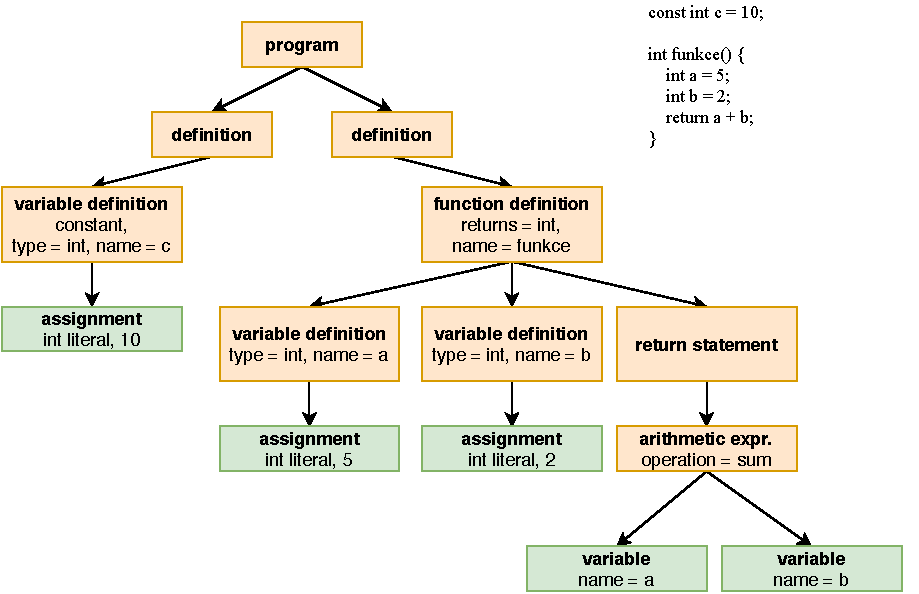
\includegraphics[width=\textwidth]{pdf/syntanalysis.pdf}}
    \caption{Abstraktní syntaktický strom}
    \label{fig:screen-transition-diagram}
\end{figure}

Generování abstraktního syntaktického stromu probíhá během zpracovávání tokenů během syntaktické analýzy. 

\subsection{Cílová platforma}
Při vyhodnocování vygenerovaného abstraktního syntaktického stromu probíhá generování instrukcí architektury PL/0.

PL/0 je jednoduchá architektura vytvořená pro vždělávací učely a procvičení konstrukcí z oblasti vytváření překladačů. Tato architektura je navržena tak, že podporuje následující instrukce:

\begin{lstlisting}[caption={Ukázka regulárních výrazů pro skenování tokenů}, captionpos=b, style=flex]
lit 0,A    uloz konstantu A do zasobniku
opr 0,A    proved instrukci A
1    unarni minus
2    +
3    -
4    *
5    div - celociselne deleni (znak /)
6    mod - deleni modulo (znak %)
7    odd - test, zda je cislo liche
8    test rovnosti (znak =)
9    test nerovnosti (znaky <>)
10    <
11    >=
12    >
13    <=
lod L,A    uloz hodnotu promenne z adr. L,A na vrchol zasobniku
sto L,A    zapis do promenne z adr. L,A hodnotu z vrcholu zasobniku
cal L,A    volej proceduru A z urovne L
int 0,A    zvys obsah top-registru zasobniku o hodnotu A
jmp 0,A    proved skok na adresu A
jmc 0,A    proved skok na adresu A, je-li na vrcholu zasobniku 0
ret 0,0    navrat z procedury (return)
\end{lstlisting}  


\begin{figure}[!ht]
    \centering
    {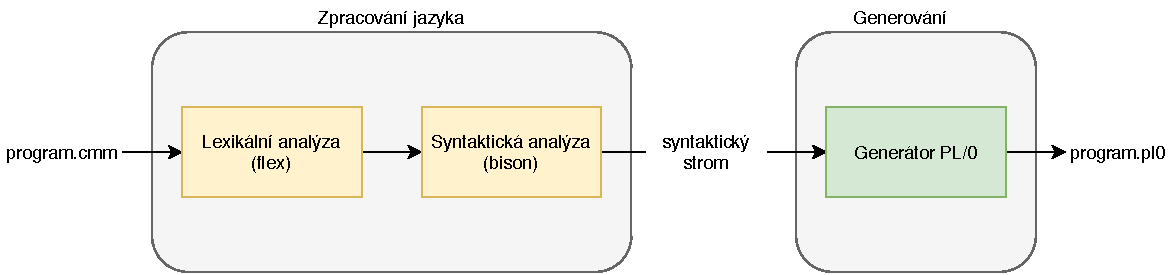
\includegraphics[width=\textwidth]{pdf/architecture.pdf}}
    \caption{Výsledná architektura navrženého překladače}
    \label{fig:screen-transition-diagram}
\end{figure}


\section{Implementace navržené architektury překladače}

Navržená architektura překladače byla implementovaná jako jeden program napsaný v jazyce C++ s využitím nástrojů \texttt{flex} a \texttt{bison}, ktere generují část programu.


\subsection{Sestavení překladače a jeho závislosti}
K sestavování vytvořeného programu jsou používány nástroje \texttt{CMake} a \texttt{make}, kdy v souboru \texttt{CMakeLists.txt} je definován postup přeložení souborů obsahující zdrojové kódy programu a závislosti na nástroje \texttt{flex} a \texttt{bison}.

Postup k sestavení podporuje kompilaci na platformách Linux a Windows, a tak je vytvořený program částečně multiplatformní.

Zdrojové kódy vygenerované nástroji \texttt{flex} a \texttt{bison} jsou umisťovány do složky \texttt{./generated}, aby byly jednoznačně odděleny od ručně psaných zdrojových kódů programu.

Úspešná kompilace končí vytvořením spustitelného programu \texttt{CMM}, který slouží k překladu programů psaných v jazyce C-{}-.


\subsection{Zpracování vstupního textu}

Předloha pro vygenerování DKA k zpracování vstupního textu a skenování tokenů se nachází v souboru \texttt{./token.l}. Při kompilaci je tento soubor přeložen pomocí nástroje \texttt{flex} a výsledný zdrojový kód DKA je vygenerován do souboru \texttt{./generated/token.c}.

Jednotlivé skenované tokeny, kterých je celkem 29, jsou definovány v souboru \texttt{./grammar.y}.

V moment rozpoznání nějakého tokenu je tento token ihned předáván další části překladače, a to konkrétně části, která má na starost syntaktickou analýzu.


\subsection{Zpracování nalezených tokenů}

Předloha pro vygenerování logiky pro zpracování nalezených tokenů se nachází v souboru \texttt{./grammar.y}. V tomto souboru se kromě seznamu skenovaných tokenů během lexikální analýzy nachází také přepsaná gramatika navrženého jazyka C-{}- v požadovaném formátu nástroje \texttt{bison}.

Během syntaktické analýzy, kdy jsou příchozí tokeny úspěšně zpracovávány podle pravidel gramatiky, jsou tyto tokeny seskupovány a dále předávány logice pro generování abstraktního syntaktického stromu.

Během kompilace překladače je pomocí nástroje \texttt{bison} vygenerován zdrojový kód do souborů začínající názvem \texttt{grammar} ve složce \texttt{./generated}.


\subsection{Vytváření abstrakního syntaktického stromu}
Při zpracování nalezených tokenů jsou vytvářeny jednotlivé prvky abstraktního syntaktického stromu. Tyto prvky jsou v kódu reprezantovány strukturou rozšiřující obecnou strukturu \texttt{ast\_node}, která definuje abstraktní funkci \texttt{evaluate} přijímající kontext vyhodnocení:

\begin{lstlisting}[caption={Struktura \texttt{ast\_node}}, captionpos=b]
struct ast_node {
    virtual ~ast_node() {
    };

    // evaluate node - for example to generate PL/0
    virtual evaluate_error evaluate(evaluate_context& context) = 0;
};
\end{lstlisting}

Každý člen syntaktického stromu je představován konkrétní strukturou dle jeho typu:

\begin{itemize}
    \item \texttt{arithmetic} -- aritmetický výraz
    \item \texttt{assign\_expression} -- přiřazení do proměnné
    \item \texttt{block} -- blok příkazů (tělo funkce, cyklu nebo podmínky)
    \item \texttt{boolean\_expression} -- booleanský výraz
    \item \texttt{command} -- struktura oblaující nějaký příkaz (např. deklaraci proměnné, výraz, definici podmínky či cyklu)
    \item \texttt{condition} -- obaluje výraz v podmínce a příkazy, které se mají provést pokud vyhodnocení podmínky bude úspěšné
    \item \texttt{declaration} -- obalující identifikátor a datový typ
    \item \texttt{expression} -- jakýkoliv výraz
    \item \texttt{for\_loop} -- obalující komponenty iteračního cyklu
    \item \texttt{function\_call} -- volání funkce
    \item \texttt{function\_declaration} -- deklarace funkce
    \item \texttt{global\_statement} -- příkaz modifikující globální rozsah (definice struktury, deklarace funkce nebo globální proměnné)
    \item \texttt{loop} -- obaluje příkazy volané uvnitř jedné iterace cyklu
    \item \texttt{program} -- kořen abstraktního syntaktického stromu, který představuje celý program
    \item \texttt{struct\_definition} -- definice struktury (obaluje jednotlivé členy této struktury)
    \item \texttt{value} -- hodnota, která bude například přiřazena nějaké proměnné
    \item \texttt{variable\_declaration} -- deklarace nové proměnné
    \item \texttt{variable\_ref} -- reference na již existující proměnnou
    \item \texttt{while\_loop} -- obalující komponenty iteračního cyklu
\end{itemize}

Následné vyhodnocení vygenerovaného stromu začíná tak, že se nad kořenem stromu zavolá funkce \texttt{evaluate}, která začne rekurzivně vyhodnocovat strom včetně jeho potomků. Během generování stromu je postupně vytvářena i tabulka symbolů, která je později využívána k překladu identifikátorů na adresy do paměti.

\subsection{Generování PL/0}
Generování instrukcí PL/0 probíhá většinou při vyhodnocování listů abstraktního syntaktického stromu, kdy se používají informace o aktuálním stavu překladu (např. tabulka symbolů, kontext). 

\begin{lstlisting}[caption={Struktura \texttt{pcode\_instruction} představující instrukci PL/0}, captionpos=b]
struct pcode_instruction {
    pcode_fct instruction;      // instruction name
    int lvl;                    // memory level
    pcode_arg arg;              // instruction argument
\end{lstlisting}
V průběhu generování jsou generované instrukce postupně přidávány do seznamu \texttt{evaluate\_context::generated\_instructions}.

\subsubsection{Přiřazování do členů struktur a jejich čtení}

Pokud mají být generovány instrukce při přístupu ke členu (nebo čtení z něj) nějaké struktury, tak se kromě vyhledání adresy začátku struktury musí i vypočítat pozice relativní k začátku struktury, kde se nachází požadovaný člen. Toto dohledávání je realizované tak, že se dle identifikátoru instance struktury vyhledá její definice. Po nalezení definice struktury, ke které přistupujeme, se iteruje po jednotlivých definicích členů struktury. Sčítáme velikosti členů, jejichž identifikátory nejsou shodné s požadovaným identifikátorem, dokud nenarazíme na požadovaný člen. Výsledná adresa relativní k začátku struktury je rovna této sumě. Při generování samotné instrukce pro zápis či čtení již specifikujeme absolutní adresu požadovaného členu.


\subsubsection{Dynamické indexování pole}

Dynamické indexování pole znamená, že index používáný pro přístup do pole není znám při překladu. Bez instrukcí \texttt{LDA} a \texttt{STA}, které načítají adresu, ke které mají přistoupit, ze zásobníku, není možné dynamické indexování realizovat. Tyto instrukce se však nenacházejí v základní instrukční sadě, a tak je třeba použít interpret PL/0, který podporuje.

Samotné generování instrukcí při indexování pole probíhá tak, že se před vložením instrukcí \texttt{STA} a \texttt{LDA}  k adrese začátku pole připočte hodnota výrazu představující index do pole. V momentě volání instrukcí \texttt{STA} a \texttt{LDA} se již v zásobníku nachází adresa ukazující na požadovaný prvek v poli daný indexem.

\subsubsection{Rozšíření interpretu \texttt{pmachine.cpp}}

Námi použitý interpret \texttt{pmachine.cpp}\footnote{\url{https://gist.github.com/gotoc/8084fd6b22892ce068f2}} nepodporuje instrukce z rožšířené instrukční sady PL/0. Pro implementaci dynamického indexování pole bylo třeba použitý interpret o tyto dvě instrukce rozšířit. Rozšíření bylo implementované přesně podle specifikace instrukcí \texttt{STA} a \texttt{LDA}.


\begin{lstlisting}[caption={Rozšíření interpretu \texttt{pmachine.cpp} o instrukce \texttt{LDA} a \texttt{STA}}, captionpos=b]
case pcode_fct::LDA: {
    auto addr = s[t];       // load address from stack
    t--;
    auto ba = base(s[t]);  // load base from stack

    s[t] = s[b + addr];     // load the value using the address and base and push it to the stack

    break;
}

case pcode_fct::STA : {
    auto addr = s[t];       // load address from stack
    t--;
    auto b = base(s[t]);    // load base from stack
    t--;
    auto value = s[t];      // load value form stack
    t--;

    s[b + addr] = value;    // store the value to the loaded address

    break;
}
\end{lstlisting}


\subsection{Vstup a výpis do konzole}
Aby bylo možné implementovat vstup a výpis do konzole, je třeba využít vestavěných funkcí interpretu. Ve zdrojovém kódu interpretu \texttt{pmachine.cpp} lze sledovat, že při zpracování instrukce \texttt{CAL} se kontroluje, zdali adresa není z oblasti definované konstantou \texttt{BuiltinBase}. Pokud ano, tak se má zavolat vestavěná funkce pro vstup či výstup do konzole.

\begin{lstlisting}[caption={Zpracování instrukce CAL v interpretu \texttt{pmachine.cpp}}, captionpos=b]
if (i.a < BuiltinBase) {
    // standard CAL instruction handler
}
else {
    int ptr;
    switch (i.a) {
        case BuiltinBase + 0:	       // consolePrintNum
            std::cout << s[t];
            break;
        case BuiltinBase + 1: ...   // consolePrintLnNum 
        case BuiltinBase + 2: ...	// consolePrintStr
        case BuiltinBase + 3: ...	// consolePrintLnStr
        case BuiltinBase + 4:        // consoleScanNum
            std::cin >> ptr;
            s[b + 3] = ptr;
            break;
    }
}
\end{lstlisting}

Před vyhodnocováním abstraktního syntaktického stromu se implicitně definují funkce \texttt{consolePrintNum}, \texttt{consolePrintLnNum}, \texttt{consolePrintStr}, \texttt{consolePrintLnStr} a \texttt{consoleScanNum}. Při jejich volání, se generují instrukce \texttt{CAL} s příslušnou adresou z báze \texttt{BuiltinBase}.


\subsection{Implementovaná rozšíření}
V rámci této semestrální práce byla implementována následující volitelná rozšíření dle zadání:

\begin{itemize}
    \item cykly \texttt{for} a \texttt{while}
    \item datový typ \texttt{boolean} a logické operace s ním
    \item datový typ \texttt{string} 
    \item násobné přiřazení (\texttt{a = b = c = d = 3;})
    \item podmíněné přiřazení / ternární operátor (\texttt{min = (a < b) ? a : b;})
    \item příkazy pro vstup a výstup (\texttt{read}, \texttt{write} - potřebuje vhodné instrukce které bude možné využít)
    \item složený datový typ (\texttt{Record})
    \item pole a práce s jeho prvky (\textbf{včetně dynamického indexování})
    \item parametry předávané hodnotou
    \item návratová hodnota podprogramu
    \item typová kontrola
\end{itemize}

\section{Závěr}	
V rámci této týmové semestrální práce byl navržen jazyk C-{}-, a následně vytvořen překladač pro tento jazyk. Během překladu jsou generovány instrukce cílové platformy PL/0. Překladač se sestává z lexikálního analyzátoru, syntaktického analyzátoru a modulu pro generování instrukcí PL/0.

Přeložené programy lze spustit v interpretu PL/0, kdy díky konstrukcím pro zápis a čtení z konzole lze tvořit interaktivní programy.

Repozitář této semestrální práce je hostovaný pomocí služby GitHub a je dostupný na adrese \url{https://github.com/topnax/kiv-fjp-sp}.


\subsection{Rozdělení práce a časová náročnost}
Práce na semestrální práci byla rozdělena následovně:
\begin{itemize}
    \item \textbf{Jindřiška Reismüllerová} (\textbf{73h}) -- dokončení přepsání gramatiky do \texttt{./grammar.y} (4h), implementace abstratkního syntaktického stromu (16h), většina generování PL/0 (38h) a implementace rozšíření (15h)
    \item \textbf{Stanislav Král} (\textbf{+55h}) -- úvodní založení CMake projektu a integrace nástrojů \texttt{bison} a \texttt{lex} (7h), lexikální analýza a úvod syntaktické analýzy (základní přepis gramatiky) (8h), zápis a čtení z pole (5h), zápis a čtení do struktur (8h), rozšíření interpretu PL/0 o instrukce \texttt{STA} a \texttt{LDA} (2h), psaní dokumentace (18h)
\end{itemize}



\section{Uživatelská příručka}
Sestavení překladače vyžaduje nainstalované nástroje \texttt{bison} a \texttt{lex}.

\newline
\noindent Postup při sestavení kompilátoru:
\begin{enumerate}
    \item spuštění příkazu \texttt{cmake .} v kořenovém adresáři projetku
    \item spuštění příkazu \texttt{make} v kořenovém adresáři projetku
    \item v kořenovém adresáři vznikl spustitelné soubory \texttt{CMM} a \texttt{pmach}
    \item \LARGE todo
\end{enumerate}

Spustitelný soubor představující překladač jazyka C-{}- do PL/0 očekává jako první argument cestu k programu k přeložení.

\newline
Přeložení souboru (výstup překladu se objeví v souboru \texttt{out.pl0}) se provádí pomocí spuštění příkazu \texttt{./CMM samples/basic.cmm}. Spuštění přeloženého C-{}- programu pomocí PL/0 interpretu: \texttt{./pmach out.plo}

    
\end{document}    
